\documentclass[conference]{IEEEtran}

\usepackage[utf8]{inputenc}
\usepackage[T1]{fontenc}
\usepackage[brazil]{babel}
\usepackage{cite}
\usepackage{graphicx}
\usepackage{booktabs}
\usepackage{array}
\usepackage{url}
\usepackage[hidelinks]{hyperref}

\begin{document}

\title{Classificação de Condições Maculares em Tomografia de Coerência Óptica com Descritores HOG e uma Rede Convolucional Compacta}

\author{\IEEEauthorblockN{Jheam Storch Ross, Felipe Mattos Vanetti de Albuquerque e Gabriel Zuany Duarte Vargas}
\IEEEauthorblockA{\textit{Departamento de Informática} \\
\textit{Universidade Federal do Espírito Santo}\\
Vitória, Brasil}}

\maketitle

% TODO: redigir resumo e palavras-chave após consolidar os resultados.

\section{Introdução}

A mácula é a região central da retina responsável pela visão de detalhes. Alterações em sua estrutura podem comprometer de forma importante a visão central, mesmo quando a visão periférica permanece preservada. Este trabalho considera as quatro classes definidas no conjunto de dados de Kermany et al.~\cite{kermany2018}: neovascularização coroideana (CNV, do inglês \textit{choroidal neovascularization}), edema macular diabético (DME, do inglês \textit{diabetic macular edema}), drusas e retina normal. Elas não correspondem a quatro doenças: CNV é um processo patológico, drusas são achados anatômicos e a classe normal é uma referência. No contexto da base, a CNV é usada como representação da forma neovascular avançada da degeneração macular relacionada à idade (DMRI), caracterizada por membrana neovascular e possível fluido sub-retiniano. O DME decorre da retinopatia diabética e apresenta espessamento da retina associado ao acúmulo de fluido intrarretiniano. Drusas são depósitos lipídicos associados à forma seca ou inicial da DMRI. A classe normal apresenta contorno foveal preservado e ausência de edema ou fluido retiniano~\cite{kermany2018,conitec2021}.

A tomografia de coerência óptica (OCT, do inglês \textit{optical coherence tomography}) é uma modalidade não invasiva e sem contato que emprega interferometria de baixa coerência para obter cortes ópticos de alta resolução dos tecidos~\cite{huang1991,bouma2022}. Durante o exame, o paciente mantém a fixação enquanto o equipamento realiza uma varredura luminosa da retina. Cada corte transversal é denominado B-scan, e uma sequência desses cortes pode compor uma representação volumétrica~\cite{bouma2022}. Em complemento ao exame clínico e à fotografia colorida de fundo de olho, a OCT permite observar separadamente as camadas retinianas e evidenciar fluido intrarretiniano ou sub-retiniano, que pode não ser claramente visível nessas outras modalidades~\cite{kermany2018}. Por isso, a OCT orienta a avaliação, o encaminhamento e o acompanhamento da resposta ao tratamento com agentes anti-VEGF (do inglês \textit{anti-vascular endothelial growth factor}).

A Fig.~\ref{fig:oct-classes} apresenta B-scans ilustrativos das quatro classes. A CNV e o DME podem produzir fluido e deformação das camadas, porém possuem mecanismos e padrões distintos; as drusas aparecem como elevações localizadas sob as camadas externas da retina; e a amostra normal preserva a depressão foveal. A presença de fluido em mais de uma condição e as diferenças entre seus padrões tornam a classificação automática um problema não trivial.

\begin{figure*}[t]
    \centering
    \setlength{\tabcolsep}{2pt}
    \begin{tabular}{cc}
        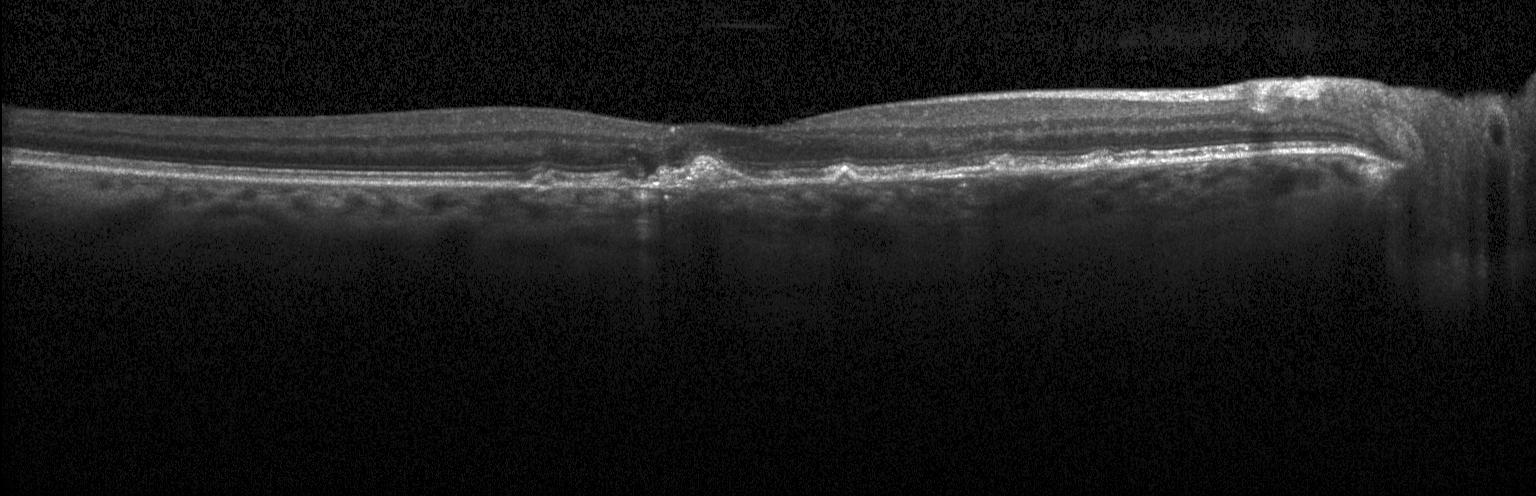
\includegraphics[width=0.49\textwidth]{figures/CNV-1676918-1.jpeg} &
        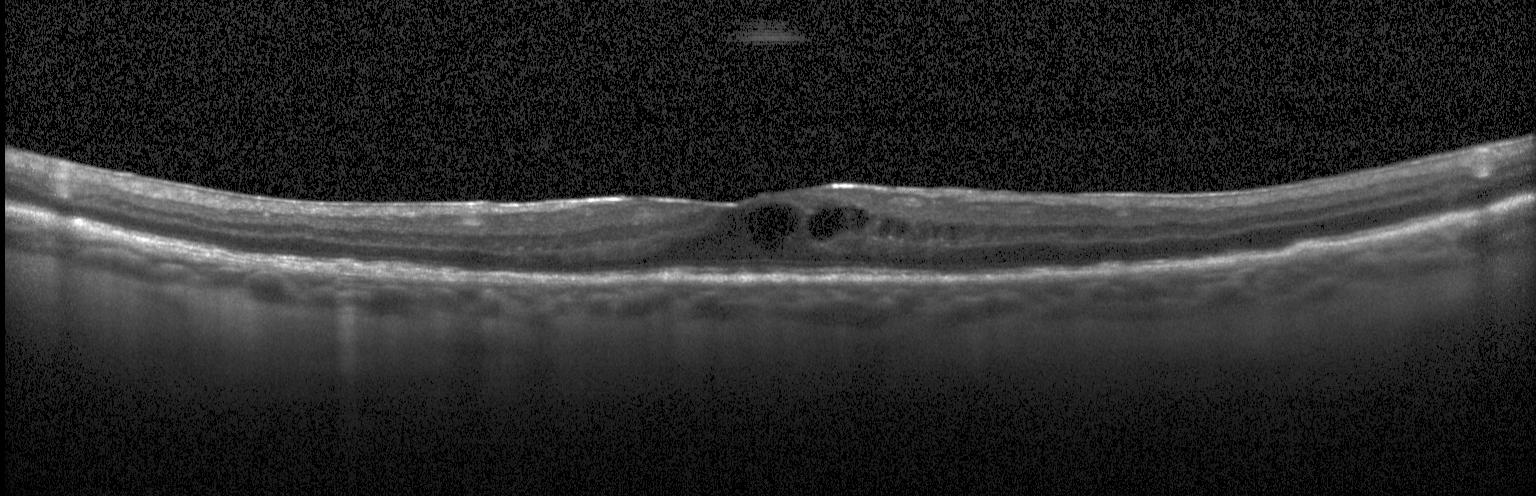
\includegraphics[width=0.49\textwidth]{figures/DME-1083927-1.jpeg} \\
        \small (a) CNV & \small (b) DME \\[1mm]
        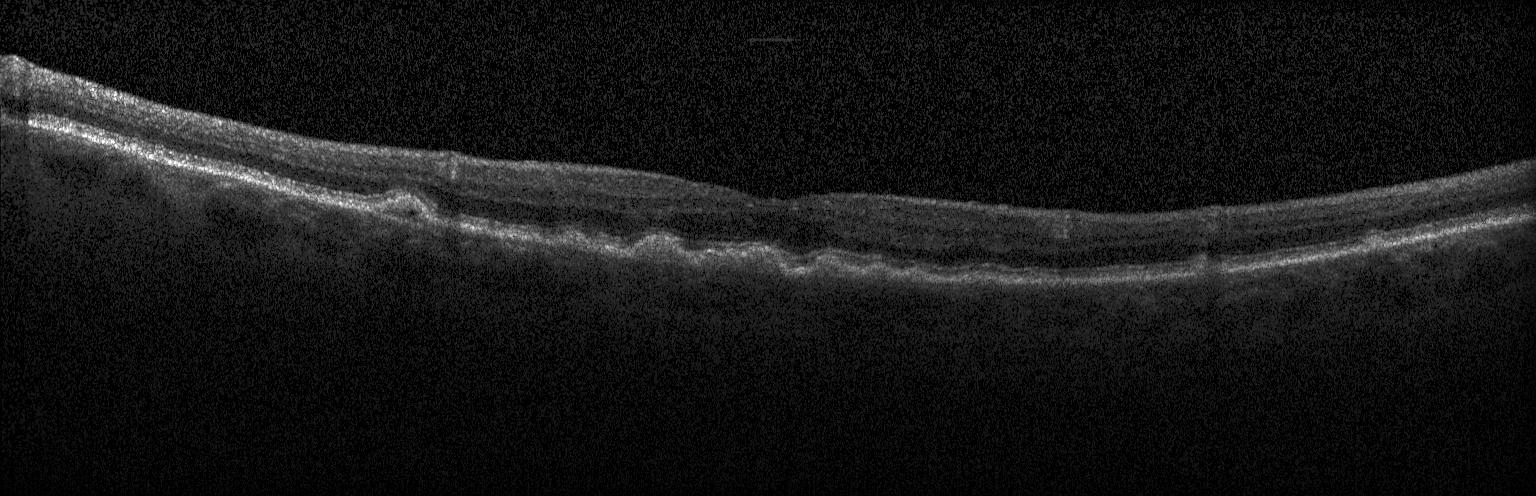
\includegraphics[width=0.49\textwidth]{figures/DRUSEN-3424668-17.jpeg} &
        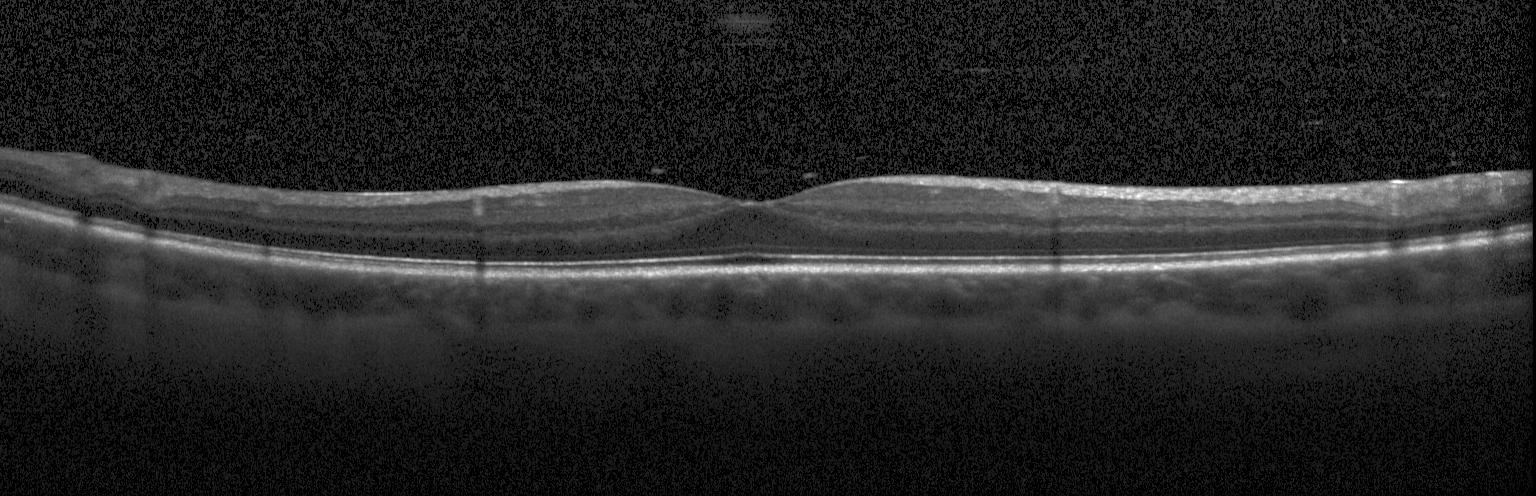
\includegraphics[width=0.49\textwidth]{figures/NORMAL-1001772-12.jpeg} \\
        \small (c) Drusas & \small (d) Normal
    \end{tabular}
    \caption{Exemplos ilustrativos das quatro classes: (a) neovascularização coroideana, (b) edema macular diabético, (c) drusas e (d) retina normal. Foram usadas as imagens de treinamento CNV-1676918-1, DME-1083927-1, DRUSEN-3424668-17 e NORMAL-1001772-12, sem recorte ou alteração de conteúdo. Fonte: versão 3 do conjunto de Kermany et al., disponibilizada sob licença CC BY 4.0~\cite{kermany_dataset}.}
    \label{fig:oct-classes}
\end{figure*}

\section{Motivação}

A deficiência visual possui impacto relevante no Brasil. A Pesquisa Nacional de Saúde de 2019 estimou que 3,4\% da população com dois anos ou mais tinha muita dificuldade ou não conseguia enxergar, totalizando 6,978 milhões de pessoas~\cite{ibge2021}. Esse indicador descreve a limitação visual autorreferida, mas não identifica suas causas e, portanto, não pode ser atribuído diretamente às condições estudadas neste trabalho. Evidência etiológica mais específica é fornecida pelo São Paulo Eye Study, realizado em uma região de renda baixa e média da cidade de São Paulo: foram examinados 3.678 participantes com 50 anos ou mais, dos quais 3.642 tiveram acuidade visual mensurável. Entre os 346 olhos com acuidade visual apresentada inferior a 20/200, doenças retinianas foram identificadas como causa principal em 35,3\%~\cite{salomao2008}. Trata-se, contudo, de uma amostra regional, não de uma estimativa nacional.

O componente diabético também representa uma população de risco expressiva. Uma revisão sistemática com 72 estudos e 29.527 adultos com diabetes estimou prevalência de retinopatia diabética de 36,28\% no Brasil, com intervalo de confiança de 95\% entre 32,66\% e 39,97\%~\cite{chagas2023}. A heterogeneidade elevada ($I^2=98\%$) exige cautela, e retinopatia diabética não equivale especificamente a DME, que pode ou não estar presente. Para pacientes acima de 60 anos com DMRI neovascular, a incorporação de aflibercepte e ranibizumabe ao Sistema Único de Saúde em 2021 reforça a relevância de identificar e acompanhar alterações tratáveis em tempo adequado~\cite{conitec2021}.

Como um exame pode conter diversos B-scans, a análise manual demanda tempo especializado. Sistemas automáticos podem apoiar a triagem e a priorização de exames para revisão especializada~\cite{kermany2018,defauw2018}. Essa função deve ser entendida como suporte à decisão: uma imagem isolada não contém histórico clínico, exame físico, informações sobre tratamento ou todas as aquisições do volume. Além disso, um modelo treinado nessa base multicêntrica internacional não está validado para uso clínico na população brasileira.

% TODO (REVISÃO): a explicação sobre os dados e a separação por paciente foi duplicada na Seção de metodologia. Cabe refletir em qual ponto do texto ela deve permanecer.
Nesse contexto, o objetivo do projeto é investigar se uma rede neural convolucional compacta, treinada do zero, consegue aprender representações úteis das quatro classes e superar uma referência clássica baseada em descritores de histogramas de gradientes orientados (HOG, do inglês \textit{histograms of oriented gradients}) e regressão logística. A comparação privilegia um protocolo reproduzível, com separação por paciente e relato conjunto de desempenho global e por classe. Foi utilizada a versão 3 do subconjunto OCT de Kermany et al.~\cite{kermany_dataset}, preservando-se o conjunto de teste oficial. A validação foi amostrada somente do conjunto de treino, em proporção de 15\%, por agrupamento dos identificadores de paciente extraídos de nomes no padrão Kermany, como \texttt{CNV-1016042-1.jpeg}. O manifesto final foi validado para garantir interseções vazias dos conjuntos de identificadores de paciente entre treino, validação e teste. O resultado pretendido é uma análise experimental de métodos de classificação, e não um dispositivo diagnóstico.

\section{Trabalhos Relacionados}

Srinivasan et al.~\cite{srinivasan2014} apresentaram um dos antecedentes mais próximos da abordagem clássica considerada neste projeto. O método extrai descritores HOG multiescala de cada B-scan e os fornece a classificadores de máquinas de vetores de suporte lineares; o rótulo do volume é determinado pela moda das previsões dos cortes. Em 45 sujeitos, divididos igualmente entre retina normal, DME e DMRI seca, o sistema identificou corretamente todos os volumes com DME e DMRI e 86,67\% dos volumes normais. O número de classes, a escala da base e a avaliação por volume diferem do presente problema, impedindo comparação direta com acurácia por B-scan.

Kermany et al.~\cite{kermany2018} estabeleceram o benchmark de quatro classes utilizado neste trabalho. Os autores adaptaram uma Inception V3 pré-treinada no ImageNet, congelaram as camadas convolucionais e treinaram uma nova camada \textit{softmax}. A acurácia multiclasse relatada foi 96,6\% em 1.000 imagens de 633 pacientes não presentes no treino. Já sensibilidade e especificidade de 97,8\% e 97,4\% foram calculadas para a decisão binária de encaminhamento urgente, não como médias das quatro classes; essas métricas não devem ser comparadas diretamente a \textit{recall} macro ou AUC multiclasse.

Trabalhos posteriores questionaram a necessidade de redes profundas pré-treinadas para esse domínio. Butola et al.~\cite{butola2020} propuseram a LightOCT, com duas camadas convolucionais e uma camada totalmente conectada, treinada do zero. Nas implementações comparativas dos próprios autores, avaliadas na partição de teste com 1.000 imagens, a LightOCT alcançou 94,5\% de acurácia, próxima de VGG-19 (93,3\%) e Inception V3 (95,8\%), mas abaixo de ResNet-101 (96,7\%). O artigo não descreve um conjunto de validação separado para essa base durante a exploração dos hiperparâmetros da LightOCT. Arefin et al.~\cite{arefin2021} também treinaram uma CNN sem transferência, formada por cinco camadas convolucionais e duas densas, e relataram 97,93\% em 968 imagens de teste, uma partição posteriormente associada à versão 2 do conjunto~\cite{tampu2022}.

Esses resultados precisam ser interpretados junto à análise de Tampu et al.~\cite{tampu2022}. Nos experimentos conduzidos pelos autores, separar B-scans sem respeitar sujeito ou volume inflou a acurácia entre 5 e 30 pontos percentuais, pois cortes consecutivos compartilham estruturas e ruído. Na versão 2 de Kermany, 92\% das imagens de teste possuíam identificadores de sujeitos também presentes no treino; na versão 3, não foi encontrada sobreposição de identificadores. Assim, o valor de Arefin et al. e outros resultados obtidos na versão 2 não constituem referências equivalentes a uma avaliação sem sobreposição por paciente.

Em uma direção mais próxima da aplicação clínica, De Fauw et al.~\cite{defauw2018} combinaram uma U-Net tridimensional, que converte o volume em mapas de tecido, com uma rede de diagnóstico e recomendação de encaminhamento. Foram usados 14.884 volumes de 7.621 pacientes, com teste em 997 pacientes. A coorte foi obtida de uma via clínica que abrangia mais de 50 condições retinianas. O sistema previa quatro níveis de encaminhamento e dez rótulos diagnósticos adicionais. Essa tarefa clínica é mais ampla que as quatro classes deste trabalho e seus resultados não são diretamente comparáveis. A Tabela~\ref{tab:related-work} resume as diferenças centrais entre os estudos comparáveis.

\begin{table*}[t]
\caption{Síntese dos trabalhos mais diretamente relacionados. Resultados de protocolos, versões e unidades de avaliação diferentes não formam um ranking único.}
\label{tab:related-work}
\centering
\footnotesize
\setlength{\tabcolsep}{4pt}
\renewcommand{\arraystretch}{1.15}
\begin{tabular}{>{\raggedright\arraybackslash}p{0.14\textwidth}
                >{\raggedright\arraybackslash}p{0.22\textwidth}
                >{\raggedright\arraybackslash}p{0.27\textwidth}
                >{\raggedright\arraybackslash}p{0.29\textwidth}}
\toprule
\textbf{Estudo} & \textbf{Abordagem} & \textbf{Dados e avaliação} & \textbf{Resultado e ressalva} \\
\midrule
Srinivasan et al.~\cite{srinivasan2014} & HOG multiescala e SVM & 45 sujeitos; normal, DME e DMRI seca; avaliação por volume & 100\% para DME/DMRI e 86,67\% para normal; tarefa menor e distinta \\
Kermany et al.~\cite{kermany2018} & Inception V3/ImageNet; convoluções congeladas & 108.312 imagens de treino; avaliação separada por paciente com 1.000 B-scans & 96,6\% de acurácia; sensibilidade/especificidade publicadas referem-se à decisão urgente \\
Butola et al.~\cite{butola2020} & LightOCT com duas convoluções, treinada do zero & Quatro classes; teste oficial com 1.000 B-scans & 94,5\%; desempenho próximo das redes pré-treinadas nas implementações dos autores \\
Arefin et al.~\cite{arefin2021,tampu2022} & CNN com cinco convoluções e duas camadas densas, sem transferência & Versão 2; teste oficial com 968 B-scans & 97,9\%; versão posteriormente associada a sobreposição entre treino e teste \\
Tampu et al.~\cite{tampu2022} & LightOCT sob diferentes estratégias de particionamento & Versões 2 e 3; divisão por imagem e por sujeito/volume & Inflação de 5--30 pontos percentuais; 92\% das imagens de teste compartilhavam ID de sujeito com o treino na versão 2; nenhum ID compartilhado foi detectado na versão 3 \\
\bottomrule
\end{tabular}
\end{table*}

Em conjunto, a literatura indica que arquiteturas compactas podem ser competitivas, mas não demonstra que transferência de aprendizado seja desnecessária em geral. Profundidade, número de parâmetros, versão da base, unidade de avaliação e estratégia de particionamento variam simultaneamente. Isso motiva a comparação controlada entre HOG e uma CNN compacta sob o mesmo manifesto com teste oficial preservado e separação validada por paciente, mantendo os experimentos exploratórios com transferência apenas como evidência secundária.

\section{Metodologia}
\label{sec:metodologia}

Esta seção descreve o protocolo experimental adotado na comparação entre os dois modelos. Inicialmente, apresentam-se o conjunto de dados e a divisão por paciente (Seção~\ref{subsec:dados}). Em seguida, descrevem-se os modelos comparados: a regressão logística sobre descritores HOG (Seção~\ref{subsec:hog_logreg}) e a rede convolucional compacta treinada do zero (Seção~\ref{subsec:cnn}). Por fim, detalham-se as estratégias que compõem o treino, comuns a ambos os modelos ou específicas da rede convolucional, a saber, o aumento de dados (Seção~\ref{subsec:aumento}), o tratamento do desbalanceamento de classes (Seção~\ref{subsec:desbalanceamento}) e a configuração de otimização (Seção~\ref{subsec:treino}), além das métricas de avaliação (Seção~\ref{subsec:metricas}).

\subsection{Dados}
\label{subsec:dados}

Foi utilizada a versão~3 do subconjunto OCT do conjunto de Kermany et al.~\cite{kermany_dataset}, formado por B-scans maculares em tons de cinza organizados nas quatro classes já apresentadas. O pacote é distribuído com uma divisão oficial entre treino e teste, sendo o teste composto por 1.000 imagens balanceadas, 250 por classe. Após a leitura das imagens e a remoção de duplicatas, o manifesto reúne 109.309 B-scans; a porção de radiografias de tórax incluída no pacote original não faz parte do escopo deste trabalho.

O conjunto de teste oficial foi preservado integralmente, sem qualquer reamostragem, para permitir comparação direta com os resultados relatados na literatura sobre a mesma partição. O conjunto de validação foi amostrado exclusivamente do treino, na proporção de 15\%, por agrupamento dos identificadores de paciente inferidos dos nomes de arquivo no padrão Kermany, como \texttt{CNV-1016042-1.jpeg}. O agrupamento mantém todas as imagens de um mesmo paciente em um único conjunto, e o manifesto foi verificado para garantir interseção vazia de identificadores entre treino, validação e teste. Essa separação é essencial, pois dividir B-scans sem respeitar o paciente infla artificialmente o desempenho; a versão~3 é adequada a esse protocolo por não apresentar sobreposição de identificadores entre treino e teste~\cite{tampu2022}.

A Tabela~\ref{tab:dataset} detalha a distribuição por classe e conjunto. No treino, as classes são acentuadamente desbalanceadas: a retina normal e a CNV concentram a maior parte das amostras, enquanto drusas e DME são minoritárias. Esse desequilíbrio motiva o tratamento descrito na Seção~\ref{subsec:desbalanceamento}. O teste oficial, ao contrário, é balanceado, com 250 imagens por classe, o que favorece a leitura das métricas globais discutidas na Seção~\ref{subsec:metricas}.

\begin{table}[t]
\caption{Distribuição de B-scans por classe e conjunto no manifesto da versão~3 do subconjunto OCT.}
\label{tab:dataset}
\centering
\footnotesize
\setlength{\tabcolsep}{5pt}
\renewcommand{\arraystretch}{1.15}
\begin{tabular}{l r r r r}
\toprule
\textbf{Classe} & \textbf{Treino} & \textbf{Validação} & \textbf{Teste} & \textbf{Total} \\
\midrule
CNV       & 32.014 &  5.191 &   250 & 37.455 \\
DME       &  9.858 &  1.490 &   250 & 11.598 \\
Drusas    &  7.408 &  1.208 &   250 &  8.866 \\
Normal    & 43.907 &  7.233 &   250 & 51.390 \\
\midrule
Imagens   & 93.187 & 15.122 & 1.000 & 109.309 \\
Pacientes &  4.067 &    718 &   635 &  5.420 \\
\bottomrule
\end{tabular}
\end{table}

\subsection{Regressão logística com HOG}
\label{subsec:hog_logreg}

A abordagem clássica combina descritores HOG com um classificador linear. Cada B-scan é convertido para tons de cinza, redimensionado para $224\times224$ e descrito por HOG com 9 orientações, células de $16\times16$ pixels e blocos de $2\times2$ células. O descritor resume a distribuição local de orientações de gradiente, sensível aos contornos das camadas retinianas alteradas pelas condições estudadas. O vetor resultante é padronizado e classificado por regressão logística multinomial (solucionador \textit{lbfgs}, limitado por 2.000 iterações), com o desbalanceamento tratado por ponderação de classes (Seção~\ref{subsec:desbalanceamento}).

\subsection{Rede Convolucional Compacta}
\label{subsec:cnn}

A rede convolucional compacta é treinada do zero e aprende representações hierárquicas diretamente dos B-scans, sem transferência de aprendizado. A Tabela~\ref{tab:cnn} apresenta sua arquitetura. As imagens, em tons de cinza, são representadas em três canais e redimensionadas para $224\times224$. O extrator de características é formado por três blocos convolucionais, cada um com convolução $3\times3$, normalização em lote, ativação ReLU e \textit{max-pooling} $2\times2$. A normalização em lote estabiliza o treino e a redução progressiva concentra a informação em mapas de características mais abstratos.

Em vez de camadas densas de grande porte, um \textit{pooling} médio global condensa cada mapa de características em um único valor, o que reduz de forma acentuada o número de parâmetros e a propensão ao sobreajuste. O vetor de 128 dimensões passa por \textit{dropout} ($p=0{,}25$) e por uma camada linear com \textit{softmax} sobre as quatro classes. O modelo totaliza cerca de 94~mil parâmetros, significativamente menor que a Inception~V3 adotada por Kermany et al.~\cite{kermany2018}, a qual possui aproximadamente 23~milhões. As estratégias de aumento de dados e de tratamento do desbalanceamento aplicadas a essa rede são descritas nas Seções~\ref{subsec:aumento} e~\ref{subsec:desbalanceamento}.

\begin{table}[t]
\caption{Arquitetura da rede convolucional compacta.}
\label{tab:cnn}
\centering
\footnotesize
\setlength{\tabcolsep}{5pt}
\renewcommand{\arraystretch}{1.2}
\begin{tabular}{l l l}
\toprule
\textbf{Camada} & \textbf{Configuração} & \textbf{Saída} \\
\midrule
Entrada & --- & $3\times224\times224$ \\
Conv+BN+ReLU & 32 filtros $3\times3$ & $32\times224\times224$ \\
\textit{MaxPool} & $2\times2$ & $32\times112\times112$ \\
Conv+BN+ReLU & 64 filtros $3\times3$ & $64\times112\times112$ \\
\textit{MaxPool} & $2\times2$ & $64\times56\times56$ \\
Conv+BN+ReLU & 128 filtros $3\times3$ & $128\times56\times56$ \\
\textit{MaxPool} & $2\times2$ & $128\times28\times28$ \\
\textit{Pooling} médio global & --- & $128$ \\
\textit{Dropout} & $p=0{,}25$ & $128$ \\
Linear + \textit{softmax} & $128 \to 4$ & $4$ \\
\bottomrule
\end{tabular}
\end{table}

\subsection{Aumento de dados}
\label{subsec:aumento}

O aumento de dados é aplicado apenas ao conjunto de treino da rede convolucional; validação e teste não são alterados. Foram utilizadas duas transformações condizentes com a natureza dos B-scans: espelhamento horizontal ($p=0{,}5$), que corresponde à simetria entre os lados nasal e temporal e à alternância entre olho direito e esquerdo, e rotação aleatória de até $5^\circ$, compatível com pequenas angulações no posicionamento do aparelho durante a aquisição. Ambas preservam a ordenação anatômica das camadas retinianas. Transformações que violariam essa ordenação foram evitadas: o espelhamento vertical, por exemplo, inverteria a sequência das camadas, colocando a coroide acima do vítreo e produzindo uma imagem sem correspondência clínica.

\subsection{Desbalanceamento de classes}
\label{subsec:desbalanceamento}

Como mostra a Tabela~\ref{tab:dataset}, o treino é desbalanceado, com razão de cerca de seis para um entre a classe mais e a menos frequente. Para evitar que as classes majoritárias dominem o aprendizado, ambos os modelos atribuem a cada classe uma importância inversamente proporcional à sua frequência, mas a aplicam de formas distintas. Na regressão logística, essa importância entra na função de perda, fazendo com que erros em classes raras pesem mais no ajuste. Na rede convolucional, ela guia a amostragem: um amostrador aleatório ponderado sorteia as imagens de cada época com reposição, exibindo com mais frequência as classes minoritárias e tornando os \textit{mini-batches} aproximadamente balanceados. Como essa reamostragem repete imagens minoritárias, é o aumento de dados (Seção~\ref{subsec:aumento}) que introduz variação entre as repetições.

\subsection{Treinamento}
\label{subsec:treino}

Os modelos foram implementados em PyTorch, com semente aleatória fixa em 42 para favorecer a reprodutibilidade. A regressão logística é ajustada em etapa única sobre os descritores HOG; o restante desta seção detalha o treino da rede convolucional. Antes de entrar na rede, cada imagem é redimensionada para $224\times224$ e normalizada com média e desvio-padrão de $0{,}5$ por canal. A rede é otimizada com Adam, taxa de aprendizado inicial de $10^{-3}$, minimizando a entropia cruzada em lotes de 32 imagens por até 50 épocas.

A taxa de aprendizado é reduzida por um fator de $0{,}2$ quando a perda de validação não melhora por duas épocas consecutivas. O treino é interrompido antecipadamente após cinco épocas sem melhora dessa perda, e o modelo correspondente à menor perda de validação é retido para avaliação no conjunto de teste oficial.

\subsection{Métricas de avaliação}
\label{subsec:metricas}

% TODO: Apresentar as métricas reportadas na próxima seção
placeholder

% TODO: inserir Resultados e Discussão, Conclusão e Agradecimentos.

\bibliographystyle{IEEEtran}
\bibliography{references}

\end{document}
